\documentclass[a5paper,titlepage,10pt,normalheadings]{scrbook}
\usepackage[a5paper,backref]{hyperref}
\usepackage[papersize={148.5mm,215mm},twoside,bindingoffset=0.5cm,hmargin={2cm,2cm},
				vmargin={2cm,2cm},footskip=1.1cm,driver=dvipdfm]{geometry}
\usepackage{palatino}
\usepackage{pstricks}
\usepackage{graphicx}
\usepackage{floatflt}
\usepackage[bahasa]{babel} 
\author{Lingkungan St. Petrus Maguwo}
\title{Warta Iman}
\setlength{\parindent}{1cm}
\psset{unit=1mm}

\newcounter{kgkcounter}[chapter]
\renewcommand{\thekgkcounter}{\arabic{kgkcounter}. }
\newcommand{\kgk}[1]{\refstepcounter{kgkcounter}\textbf{\flushleft \textbf{\thekgkcounter #1}}\\}

\hyphenation{pe-sa-wat-pe-sa-wat}
\hyphenation{Scho-ol}
\hyphenation{Ho-ge}
\hyphenation{sung-g uh}

\begin{document}
\thispagestyle{empty}
\newcommand{\edisi}[1]{%
\DeclareFixedFont{\PT}{T1}{ppl}{b}{}{0.7in}
\DeclareFixedFont{\PTit}{T1}{ppl}{b}{it}{0.7in}
\DeclareFixedFont{\PTsmall}{T1}{ppl}{b}{it}{0.25in}
\DeclareFixedFont{\PTsmaller}{T1}{ppl}{b}{it}{0.175in}
\DeclareFixedFont{\PTsmallest}{T1}{ppl}{b}{it}{0.15in}

\begin{pspicture}(14cm,2cm)
\rput[rb](10.35cm,3cm){\PTsmallest {#1}}
\rput[lb](-2cm,1.5cm){\PT {WARTA IMAN}}
\rput[lb](0cm,0.5cm){\PTsmall {Lingkungan St. Petrus Maguwo}}
\end{pspicture}%
}

\newcounter{kgkcounter}[chapter]
\renewcommand{\thekgkcounter}{\arabic{kgkcounter}. }
\newcommand{\kgk}[1]{\refstepcounter{kgkcounter}\textbf{\flushleft \textbf{\thekgkcounter #1}}\\}

\newcommand{\kutipan}[1]{%
\noindent{\framebox{\parbox{10cm}{\centering\emph{#1}}}}}

\edisi{November 2011}

%\vspace{1cm}

\begin{center}
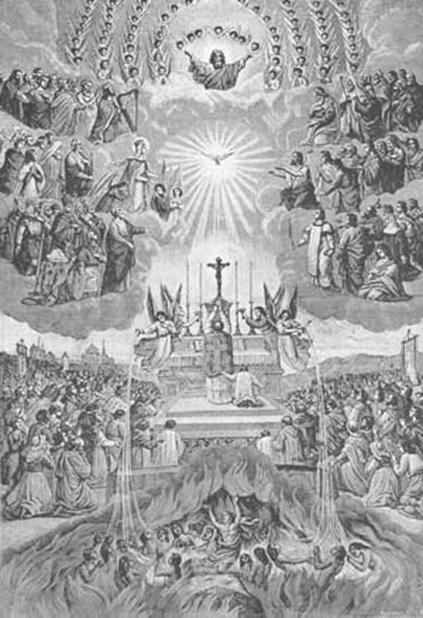
\includegraphics[scale=0.85]{gambar/purgatory2.jpg}
\end{center}

%\vspace{1cm}

\begin{center}
{\PTsmaller {Kasih, kerendahan hati, dan menurut pada kehendak Allah }}
\end{center}

\newpage

\section*{\center Dari Redaksi}

\indent{Berkah Dalem,}

Setelah beberapa saat Warta Iman (WI) tidak muncul, mulai bulan Agustus 2011 WI akan diusahakan mengunjungi Anda sekali dalam 1 bulan. Bulan Agustus mengingatkan kita pada peringatan hari kemerdekaan Republik Indonesia yang jatuh pada tanggal 17 Agustus. Oleh karena itu tema untuk bulan ini adalah kemerdekaan. 
Sejak semula ternyata memang putra-putra gereja, khususnya dari Keuskupan Agung Semarang turut menghiasi pusara ibu pertiwi dengan jasa-jasanya. Setidaknya ada Ignatius Slamet Riyadi (1945), Agustinus Adisucipto (1947), dan Yos Sudarso (1961). Kisah-kisah mengenai mereka dapat kita simak pada beberapa tulisan di edisi kali ini.

Bulan Juli kemarin beredar juga Buletin Kasih sebagai rasa syukur pesta nama St. Petrus yang jatuh pada tanggal 29 Juni. Rasa syukur pula yang menyebabkan anak-anak muda (OMK) St. Petrus giat berlatih gamelan dan mempersembahkan hasilnya pada misa syukur pada tanggal 3 Juli 2011. Saudara Ferry mewakili teman-temannya menuliskan pengalamannya nabuh gamelan. Dalam tulisannya Ferry mengajak generasi muda untuk mensyukuri kemerdekaan dan mengisinya dengan kegiatan bersama dengan kebersamaan.

Tulisan tentang kasih yang membebaskan dan kemerdekaan manusia dari beban hukum dapat memperkaya kita tentang hubungan kasih dan kebebasan. Edisi kali inipun dihiasi oleh puisi agar banyak aksi daripada banyak bicara kiriman dari BS. 

Mulai edisi ini akan dicuplik tentang isi Kompendium Katekese Gereja Katolik, yang diharapkan dapat memperkaya pengetahuan iman kita.

\begin{center}***\end{center} 

\vspace*{1.3cm}

\noindent{\framebox{\parbox{10cm}{\scriptsize
Warta Iman\\
Media komunikasi dan informasi umat lingkungan St. Petrus\\
Alamat Redaksi: Lingkungan St. Petrus Maguwo\\
E-mail: stpetrusmgw@gmail.com
}}}

\newpage
\section*{Ignatius Slamet Riyadi: Teladan dari Solo}
\begin{floatingfigure}[r]{2cm}
\begin{center}
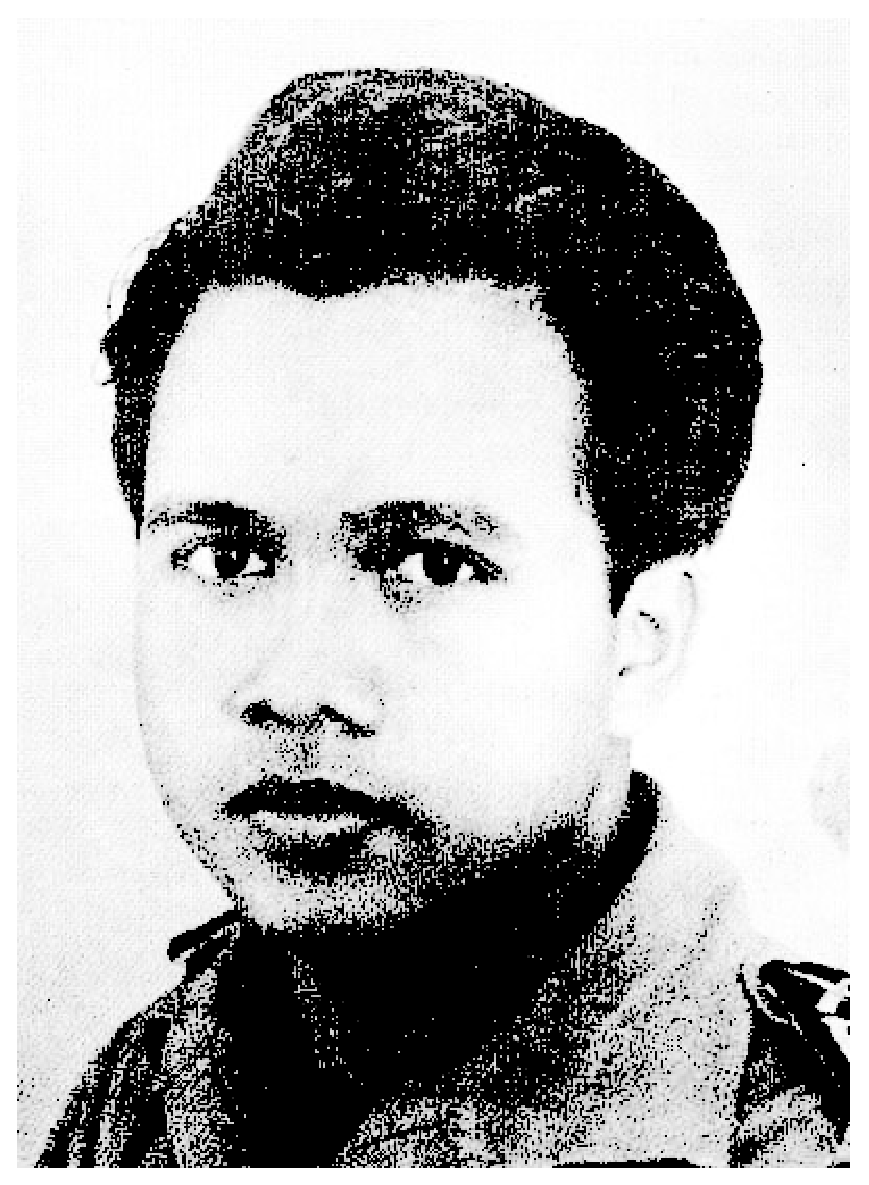
\includegraphics[scale=0.15]{Slamet-riyadi.ps}
\end{center}
\end{floatingfigure}
Salah satu tokoh pahlawan nasional yang berasal dari Solo adalah Ignatius Slamet Riyadi. Sesuai dengan namanya beliau adalah seorang Katolik yang ikut dalam perjuangan kemerdekaan Indonesia. 
Namanya digunakan sebagai nama jalan utama di jantung kota Solo tempat kelahirannya.   
Anak dari Idris Prawiropralebdo, seorang perwira anggota legium Kasunanan Surakarta, yang lahir 26 Juli 1927 ini sangat menonjol kecakapan dan keberaniannya, terutama setelah Jepang bertekuk lutut dan kemerdekaan Indonesia diproklamasikan. 

Ignatius Slamet Rijadi adalah salah seorang di antara ribuan anak muda yang sejak detik pertama Proklamasi Kemerdekaan Indonesia secara sukarela terjun memenuhi panggilan revolusi. Sebagai bekas bintara Kaigun (Angkatan Laut Jepang) yang batal dikirim ke Tokyo karena Perang Pasifik berakhir lebih cepat, Slamet Rijadi kemudian tampil memimpin aksi penyerbuan ke markas Kempeitai (Polisi Rahasia Jepang) di Solo dan menjadi anak zaman. Pertempuran demi pertempuran dilalui Slamet Rijadi, dari mengusir Jepang, melawan Inggris, Belanda, pemberontak Komunis, dan Darul Islam, hingga menumpas Republik Maluku Selatan. Dia gugur pada usia 23 tahun dengan pangkat Letnan Kolonel sebagai Komandan Operasi Maluku Selatan akibat tembakan seorang sniper di depan Fort Victoria, Ambon, Maluku. Sebutan Pahlawan Nasional sekaligus anugerah Bintang Mahaputera Adipradana kepada Brigadir Jenderal (Anumerta) Ign. Slamet Rijadi disampaikan oleh Presiden Susilo Bambang Yudhoyono awal November 2007 \textit{"untuk tindak kepahlawanan dalam perjuangan merebut, membela dan mempertahankan negara dan bangsa, sehingga bisa jadi teladan bagi seluruh masyarakat Indonesia."}

\subsection*{Kepahlawanan}

Pada suatu peristiwa saat akan diadakannya peralihan kekuasaan di Solo oleh Jepang yang dipimpin oleh Tyokan Watanabe yang merencanakan untuk mengembalikan kekuasaan sipil kepada kedua kerajaan yang berkedudukan di Surakarta, yaitu Kasunanan dan Praja Mangkunagaran, akan tetapi rakyat tidak puas. Para pemuda telah bertekad untuk mengadakan perebutan senjata dari tangan Jepang, maka rakyat mengutus Muljadi Djojomartono dan dikawal oleh pemuda Suadi untuk melakukan perundingan di markas Ken Pei Tai (polisi militer Jepang) yang dijaga ketat. Tetapi sebelum utusan tersebut tiba di markas, seorang pemuda sudah berhasil menerobos kedalam markas dengan meloncati tembok dan membongkar atap markas Ken Pei Tai, tercenganglah pihak Jepang, pemuda itu bernama Slamet Riyadi.


\subsection*{Karir militer}

Pada tahun 1940, ia menyelesaikan pendidikan di HIS, ke Mulo Afd. B dan kemudian dilanjutkan ke Pendidikan Sekolah Pelayaran Tinggi, dan memperoleh ijasah navigasi laut dengan peringkat pertama dan mengikuti kursus tambahan dengan menjadi navigator pada kapal kayu yang berlayar antar pulau Nusantara. Setelah pasukan Jepang, mendarat di Indonesia melalui Merak, Indramayu dan dekat Rembang pada tanggal 1 Maret 1942 dengan kekuatan 100.000 orang, dan walaupun memperoleh perlawanan dari Hindia Belanda,  tetapi dalam waktu singkat yaitu pada tanggal 5 dan 7 Maret 1942,  Kota Solo dan Yogyakarta jatuh ketangan Jepang.

Slamet Riyadi merasa terpanggil membela ibu pertiwi, dan menjelang proklamasi 1945,  ia mengobarkan pemberontakan dan melarikan sebuah kapal kayu milik Jepang, usaha Ken Pei Tai untuk menangkapnya tidak pernah berhasil,  bahkan setelah Jepang bertekuk lutut. Slamet Rijadi berhasil menggalang para pemuda, menghimpun kekuatan pejuang dari pemuda-pemuda terlatih eks Peta/Heiho/Kaigun dan merekrutnya dalam kekuatan setingkat Batalyon,  yang dipersiapkan untuk mempelopori perebutan kekuasaan politik dan militer di kota Solo dari tangan Jepang ( Slamet Riyadi diangkat sebagai Komandan Batalyon Resimen I Divisi X ).

Dalam perkembangannya terjadi pergantian pimpinan militer,  Divisi X dirubah menjadi Divisi IV, dengan Panglimanya Mayor Jenderal Soetarto dan divisi ini dikenal dengan nama Divisi Penembahan Senopati, yang membawahi 5 Brigade tempur . Diantaranya Brigade V dibawah pimpinan Suadi dan mempunyai Batalyon XIV dibawah komando Mayor Slamet Rijadi,  yang merupakan kesatuan militer yang dibanggakan. Pasukannya terkenal dengan sebutan anak buah "Pak Met" . Selama agresi Belanda II,  pasukannya sangat aktif melakukan serangan gerilya terhadap kedudukan militer Belanda, pertempuran demi pertempuran membuat sulit pasukan Belanda dalam menghadapi taktik gerilya yang dijalankan Slamet Riyadi. 

Namanya mulai disebut-sebut karena hampir di-setiap peristiwa perlawanan di kota Solo selalu berada dalam komandonya.

Sewaktu pecah pemberontakan PKI-Madiun, batalyon Slamet Rijadi sedang berada diluar kota Solo, yang kemudian diperintahkan secara langsung oleh Gubernur Militer II - Kolonel Gatot Subroto untuk melakukan penumpasan ke arah Utara, berdampingan dengan pasukan lainnya, operasi ini berjalan dengan gemilang.

Dalam palagan perang kemerdekaan II, Slamet Rijadi dinaikkan pangkatnya menjadi Letnan Kolonel, dengan jabatan baru Komandan "Wehrkreise I" ( Penembahan Senopati )yang meliputi daerah gerilya Karesidenan Surakarta, dan dibawah komando Gubernur Militer II pada Divisi II,  Kolonel Gatot Subroto. Dalam perang kemerdekaan II inilah Let.Kol. Slamet Rijadi, membuktikan kecakapannya sebagai prajurit yang tangguh dan sanggup mengimbangi kepiawaian komandan Belanda lulusan Sekolah Tinggi Militer di Breda Nederland. Siang dan malam anak buah Overste (setingkat Letnan Kolonel ). Van Ohl digempur habis-habisan, dengan penghadangan, penyergapan malam, sabotase . Puncaknya ketika Let.Kol Slamet Riyadi mengambil prakarsa mengadakan "Serangan Umum Kota Solo" yang dimulai tanggal 7 Agustus 1949, selama empat hari empat malam. Serangan itu membuktikan kepada Belanda, bahwa gerilya bukan saja mampu melakukan penyergapan atau sabotase, tetapi juga mampu melakukan serangan secara frontal ketengah kota Solo yang dipertahankan dengan pasukan kavelerie, persenjataan berat-artileri, pasukan infantri dan komando yang tangguh. Dalam pertempuran selama empat hari tersebut, 109 rumah penduduk porak poranda, 205 penduduk meninggal karena aksi teror Belanda,  7 serdadu Belanda tertembak dan 3 orang tertawan sedangkan dipihak TNI 6 orang gugur.

Setelah terjadi gencatan senjata,  dan pada waktu penyerahan kota Solo kepangkuan Republik Indonesia,  dari pihak Belanda diwakili oleh "Overste Van Ohl" sedangkan dari pihak R.I oleh Let.Kol. Slamet Riyadi. Ov.Van Ohl demikian terharu, bahwa Let. Kol. Slamet Riyadi yang selama ini dicari-carinya ternyata masih sangat muda . " Oooh ...Overste tidak patut menjadi musuh-ku.....", Overste pantas menjadi anakku, tetapi kepandaiannya seperti ayahku.

Pada akhir tahun 1949, sebagai penganut agama Katolik, Slamet Riyadi di baptis dengan nama Ignatius di Gereja Santo Antonius Purbayan Solo. Pada tanggal 10 Juli 1950, Letnan Kolonel Ignatius Slamet Rijadi, berangkat dengan kapal Waikalo dan memimpin batalyon 352 untuk bergabung dengan pimpinan umum operasi - Panglima TT VII - Kolonel Kawilarang, dalam penugasan menumpas pemberontakan Kapten Andi Aziz di Makasar dan pemberontakan Republik Maluku Selatan (RMS) yang dipelopori oleh Dr. Soumokil dan kawan-kawan.

\subsection*{Riwayat Perjuangan}

\begin{tabular}{cp{9cm}}
1940&Sekolah Tinggi Pelayaran Rekrutmen Pemuda oleh tentara Jepang\\ 
1943&Navigator kapal kayu Pemberontakan kapal,milik Jepang \\
1945&Dan.Yon.Res.I, Divisi I Perang di Krsd. Solo melawan Jepang \& Belanda\\ 
1945&Dan.Yon.Res.I, Divisi I Penumpasan pemberontakan PKI Madiun \\
1948&Dan.Wehrkreise I Perang Kemerdekaan II, Serangan Umum Solo \\
1949&Wakil Pemerintah RI Penyerahan Kota Solo \\
1949&Komando Yon.352 Mendukung Div.Siliwangi menumpas APRA di Jabar.\\ 
1949&Wakil.Panglima TT VII. Penumpasan Pemberontakan di Makasar, RMS Ambon \\
1950&Wakil.Panglima TT VII. \\
1950&Gugur di gerbang benteng Victoria, Ambon 4-11-1950 \\

1950&Brigadir Jendral Anumerta Kenaikan pangkat atas jasa almarhum\\ 
2007&mendapat penghormatan sebagai Pahlawan Nasional. \\
2007&dibangun Patung Ignatius Slamet Riyadi di bundaran Gladak, Solo.\\
\end{tabular}

\vfill
\noindent{
\framebox{\parbox{10cm}{\emph{
\textbf{Dua perintah cinta kasih}
\begin{enumerate}
\item Kasihilah Tuhan Allahmu dengan segenap hatimu, dengan \\segenap jiwamu,
dan dengan segenap akal budimu.
\item Kasihilah sesamamu seperti dirimu
sendiri.
\end{enumerate}
}}}}

\newpage
\section*{Agustinus Adisutjipto: Bapak Penerbang Indonesia}

\begin{floatingfigure}[l]{2cm}
\begin{center}
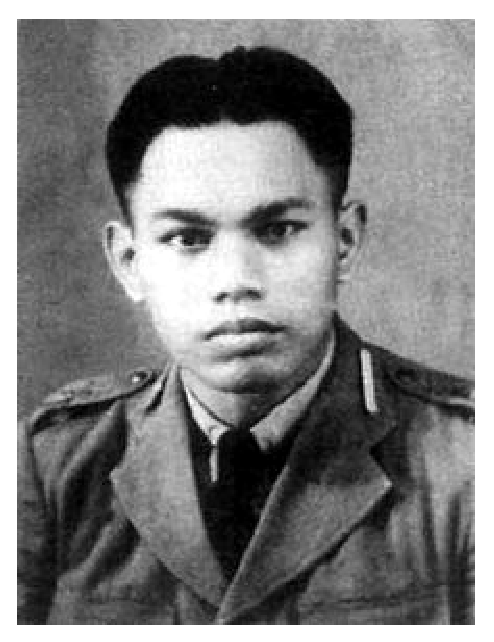
\includegraphics[scale=0.25]{Adisutjipto.ps}
\end{center}
\end{floatingfigure}
Lahir di Salatiga, Jawa Tengah, 3 Juli 1916 - meninggal di Bantul, Yogyakarta 29 Juli 1947 pada umur 31 tahun. Beliau adalah seorang Katolik, pahlawan nasional, dan seorang komodor udara Indonesia

Agustinus Adisutjipto sempat belajar di Sekolah Tinggi Kedokteran (Geneeskundige Hoge School) di Jakarta, tetapi tidak selesai. Kemudian ia memutuskan untuk pindah ke Sekolah Penerbang Militaire Luchtvaart di Kalijati. Selesai pendidikan ia bertugas di Squadron Pengintai Udara.

Sesudah Indonesia merdeka, ia menyumbangkan tenaga membina Angkatan Udara Republik Indonesia bersama S. Suryadarma, yang kemudian diangkat menjadi Kepala Staf AURI. Saat itu, tenaga penerbang sangat sedikit. Pesawat terbang hampir-hampir tidak ada, dan kalau pun ada sudah rongsokan. Teknisi-teknisi Indonesia berusaha memperbaiki pesawat tersebut. Tanggal 27 Oktober 1945, Adisutjipto berhasil menerbangkan sebuah pesawat. Penerbangan itu adalah penerbangan pertama yang dilakukan oleh putra Indonesia. Pada tanggal 1 Desember 1945 Adisutjipto mendirikan Sekolah Penerbang di Yogyakarta, tepatnya di Lapangan Udara Maguwo, yang kemudian diganti namanya menjadi Bandara Adisucipto, untuk mengenang jasa beliau sebagai pahlawan nasional. Di situ dididik kader-kader Angkatan Udara. Karena jasa-jasanya itu Adisutjipto disebut bapak Penerbang Indonesia.

Jabatan lain yang pernah dipegangnya ialah Wakil II Kepala Staf Angkatan Udara. Selain itu, pernah pula ditugasi ke India dan Filipina untuk mencari tenaga pelatih dan menyewa pesawat terbang. Di India, berkat bantuan Perdana Menteri Jawaharlal Nehru, ia berhasil mengadakan perundingan dengan Patnaik yang kemudian bersedia menyewakan sebuat pesawat Dakota.

Agustinus Adisutjipto adalah pribadi yang mempunyai komitmen tinggi terhadap negara dan bangsa. Komitmen itu tidak lepas dari hidup imannya yang kuat. Iman kepada Kristus telah menggerakkan hidupnya untuk melayani dan mengabdi kepada sesama bangsa dan negara meski risiko besar harus ditanggung.

{\small Marsekal Muda (Pur) Agustinus Adisutjipto akrab dipanggil Cip namun kemudian rekan-rekannya memanggilnya Pak Adi merupakan putra pertama dari lima bersaudara buah perkawinan Roewidodarmo dan Latifatun. Adisutjipto, sangat gemar bermain sepakbola, naik gunung, tenis dan catur. Intelektualitasnya terasah lewat hobinya membaca buku-buku kemiliteran dan filsafat. Pribadinya dikenal pendiam, namun sangat reaktif bila harga dirinya terinjak. Ketika Jepang mendarat Maret 1942, peta penerbangan Hindia Belanda berubah. Adisutjipto yang ketika PD II pecah ditempatkan di skadron intai di Jawa beserta rekan-rekannya seperti Sujono, Sulistyo, dan Husein Sastranegara, tidak pernah lagi terbang. Semua yang berbau Belanda dimusnahkan. Untuk mengisi kekosongan, Cip bekerja di perusahaan angkutan bus milik Jepang.

Sejak pekik kemerdekaan berkumandang 17 Agustus 1945, satu demi satu muncul berbagai tuntutan. Termasuk penerbangan militer. Suryadarma bertindak cepat. Para eks penerbang AU Hindia Belanda, seperti Adisutjipto, dipanggilnya. Berbagai langkah konsolidasi, mulai dari mengumpulkan ratusan pesawat sampai mengupayakan perbaikan pesa-wat-pesawat peninggalan Jepang, diambil.

Usaha Suryadarma langsung berbuah. Buktinya, Adisutjipto berhasil menerbangkan pesawat Nishikoren dari Cibereum ke Maguwo, 10 Oktober 1945. Peristiwa ini tercatat sebagai penerbangan pertama di wilayah RI merdeka oleh awak Indonesia. Tujuhbelas hari kemudian, kembali Adisutjipto membakar semangat perjuangan dengan menerbangkan pesawat Cureng bertanda merah putih. Peristiwa ini mengukir lagi catatan sejarah, sebagai penerbangan berbendera merah putih pertama di tanah air.

Adi Sutjipto terbang ke India untuk mengambil obat2an dan sekembalinya dari India ketika memasuki wilayah Indonesia. Di ujung cakrawala, terlihat pesawat Dakota VT-CLA melakukan approach. Para penumpangnya, Adisutjipto, Abdulrachman Saleh, AN Constantine (pilot), R Hazelhurst (ko-pilot), Adisumarmo Wiryokusumo (engineer), Bhida Ram, Nyonya Constantine, Zainal Arifin (wakil dagang RI), dan Gani Handonocokro, tentu bahagia karena sesaat lagi akan mendarat. Begitu juga Sudarjono yang lagi piket, akan bertemu dengan kakaknya.

Sekonyong-konyong, muncul dua pesawat P-40 Kitty Hawk Belanda dari arah utara yang langsung memberondong Dakota, pesawat sipil yang jelas-jelas membawa bantuan. Pesawat kehilangan ketinggian, melayang kencang dan menyambar sebatang pohon hingga badannya patah menjadi dua bagian. Begitu pesawat terhempas ke tanah, langsung terbakar. Suryadarma dan semua orang penunggu, berlarian ke arah pesawat naas.
Peristiwa itu terjadi di Dusun Ngoto pada tanggal 29 Juli 1947. Beliau dimakamkan di pemakaman umum Kuncen I dan II, dan kemudian pada tanggal 14 Juli 2000 dipindahkan ke Monumen Perjuangan di Desa Ngoto, Bantul, Yogyakarta.
}
\newpage
\section*{Laksamana Madya Yosaphat Sudarso: Berkorban untuk keselamatan teman} 

\begin{floatingfigure}[r]{2cm}
\begin{center}
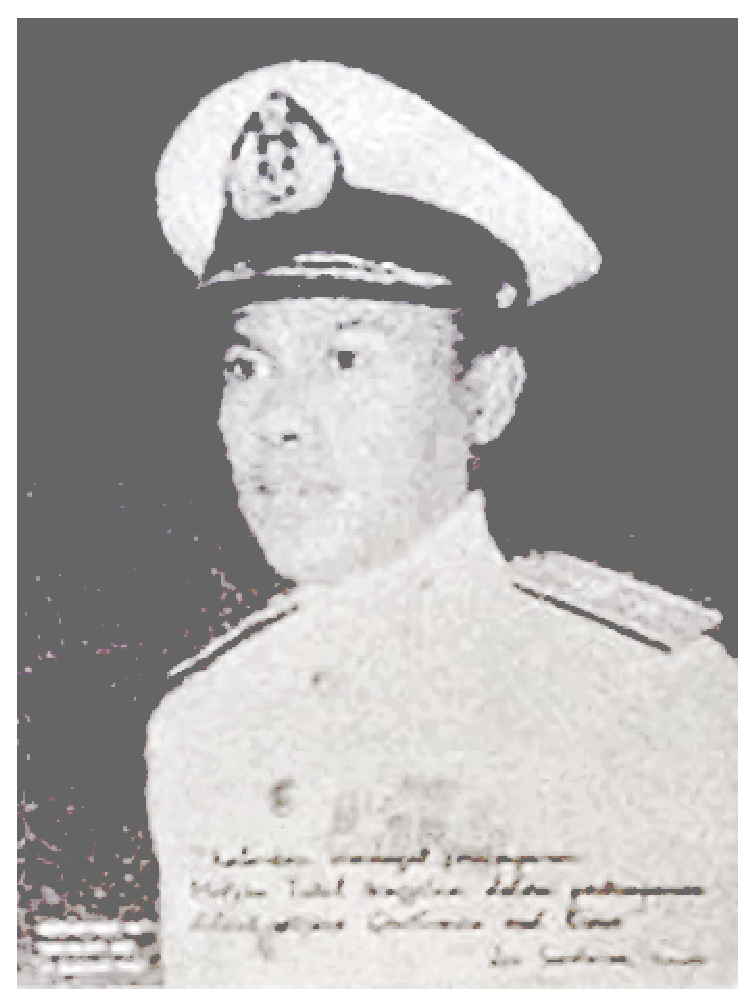
\includegraphics[scale=0.175]{Yos-Sudarso.ps}
\end{center}
\end{floatingfigure}
Laksamana Madya Yosaphat Soedarso atau yang lebih dikenal dengan nama Yos  Sudarso adalah pahlawan nasional Indonesia yang dilahirkan di Salatiga, Jawa  Tengah, 24 November 1925 dan pernah menjabat sebagai Kepala Staff Angkatan Laut.  Meski sebagai orang nomor satu di TNI AL, ia bukanlah tipe pemimpin yang berdiam diri di belakang meja.  Di usianya yang masih muda 36 tahun, ia turut ke medan tempur maju ke garis depan untuk merebut Irian Barat dari kolonial Belanda. Di atas KRI Macan Tutul di Laut Aru, Yos Sudarso gugur dengan berani.

Pertempuran Laut Aru adalah suatu pertempuran yang terjadi di Laut Aru, Maluku, pada tanggal 15 Januari 1962 antara Indonesia dan Belanda. Insiden ini terjadi sewaktu dua kapal jenis destroyer, pesawat jenis Neptune dan Frely milik Belanda menyerang KRI Macan Tutul, KRI Macan Kumbang dan KRI Harimau milik Indonesia yang sedang berpatroli pada posisi 04,49° LS dan 135,02° BT. Komodor Yos Sudarso gugur pada pertempuran ini setelah menyerukan pesan terakhirnya yang terkenal, "Kobarkan semangat pertempuran".

Pada saat itu terjadi pertempuran sengit antara pasukan militer Indonesia  dengan Belanda. Meski berstatus sebagai Kepala Staff TNI-AL Yos sudarso ikut  turut ke medan tempur. Naas dalam peristiwa tersebut, Laksamana Madya Yos  Sudarso gugur setelah KRI Macan Tutul di bombardir Belanda di Laut Aru saat  melawan armada Belanda.

Armada Indonesia di bawah pimpinan Yos Sudarso, yang saat itu berada di KRI Macan Tutul, berhasil melakukan manuver untuk mengalihkan perhatian musuh sehingga hanya memusatkan penyerangan ke KRI Macan Tutul. KRI Macan Tutul tenggelam beserta awaknya, tapi kedua kapal lainnya berhasil selamat.

Beliau gugur di atas KRI Macan Tutul dalam pertempuran Laut Aru pada masa kampanye Trikora. Namanya kini diabadikan pada sebuah KRI dan pulau. Ia gugur di atas KRI Macan Tutul pada tanggal 13 Januari  1962 pada saat berusia 36 tahun. Keikutsertaannya dalam posisi sebagai KSAL-pun  dipertanyakan karena tidak lazimnya seorang Kepala Staff Angkatan Laut turun  langsung dalam medan tempur.

Untuk menghargai jasa-jasa atas keikutsertaannya dalam memperjuangkan merebut Irian  Barat, ia dianugerahi sebagai Pahlawan Pembela Kemerdekaan. Kini namanya  diabadikan sebagai nama armada angkatan laut Indonesia, nama pulau, dan nama  jalan-jalan protokol di kota-kota besar Indonesia.

Ia meninggalkan seorang istri bernama Ny. Siti Kustini, yang dinikahinya pada  tahun 1955 dan dikaruniai lima anak dan dua diantaranya meninggal dunia.

Berselang 44 tahun setelah Yos Sudarso meninggal. Istri pahlawan Aru ini, Nyonya Josephine F Siti Kustini kemudian meninggal. Siti Kustini yang merupakan kelahiran Ngawi, Jawa  Timur, 1935, meninggal dunia pada usia 71 tahun tepatnya, Sabtu 2 September  2006 pukul 14.00, di Rumah Sakit Angkatan Laut Dr Mintohardjo, Jakarta. Akibat penyakit jantung dan radang paru-paru. Jenazah  kemudian dimakamkan, Senin, 4 September 2006 di Tempat Pemakaman Umum Kaliwuluh,  Desa Kaliwuluh, Kecamatan Kebak Kramat, Kabupaten Karanganyar, Jawa Tengah.

Semasa hidupnya, Ny. Siti Kustini dikenal sebagai orang yang sangat disiplin, selalu tepat  waktu, termasuk menunaikan ibadah agama dengan mengikuti misa kudus hampir  setiap hari.

Sebelum pemberangkatan jenazah dari Jakarta menuju Surakarta dengan menggunakan pesawat TNI AL dari Bandar Udara Halim Perdanakusuma. Misa arwah terlebih dahulu dilakukan yang dipimpin Pastor Luarens di kediaman almarhumah, di jalan  Cimandiri Nomor 12, Cikini, Jakarta Pusat. Saat itu juga dihadiri mantan Kepala  Staf TNI Angkatan Laut Laksamana (Purn) Sudomo, mantan Gubernur DKI Jakarta Ali  Sadikin, dan sesepuh TNI AL lainnya





\vfill
\noindent{
\framebox{\parbox{10cm}{\emph{
\textbf{Tujuh karya amal kasih rohani}
\begin{enumerate}
\setlength{\itemsep}{0pt}
\item Menasihati orang yang ragu-ragu.
\item Mengajar orang yang belum tahu.
\item Menegur pendosa.
\item Menghibur orang yang menderita
\item Mengampuni orang yang menyakiti.
\item Menanggung kesalahan dengan sabar.
\item Berdoa untuk orang yang hidup dan yang mati.
\end{enumerate}
}}}}



\newpage
\section*{Sepenggal Kisah dari OMK Ling. St.Petrus}
\subsection*{\emph{Oleh Yacintha Ferry Kurnia}}

Beberapa bulan yang lalu lingkungan St.Petrus baru saja merayakan pesta nama pelindung, untuk memeriahkan acara tersebut OMK St. Petrus, yang memang saat itu sedang memiliki program untuk melestarikan musik tradisional Jawa, yaitu Gamelan, diberi kesempatan untuk tampil perdana memainkan gamelan mengiringi misa pada perayaan pesta nama di gereja Bunda Maria Maguwo. 

	Begitu banyak kisah dibalik penampilan perdana mereka. Mulai dari mereka telat datang latihan hingga masalah baju surjan yang kegedean. Namun itu semua tidak menghalangi kami untuk berkarya dan menunjukkan yang terbaik. Awalnya ketua mudika kami sempat sedikit putus asa karena hanya sedikit yang ingin berpartisipasi bermain gamelan ini. Namun setelah latihan hari pertama dengan hanya beberapa orang namun sudah cukup membuat orangtua kami begitu terpana. Diantara kami hanya 3 orang saja yang memang sudah menguasai gamelan dan yang lainnya semua mulai dari nol. Bagi sebagian orang mungkin cukup mengejutkan.  Namun itulah kami, he he $\ldots$ $\ddot\smile$

	Setelah melalui proses latihan yang bisa dibilang begitu singkat, akhirnya tibalah saat kami menunjukkan hasil kerja keras kami berlatih selama beberapa minggu. Cukup grogi untuk kami, namun semuanya itu sirna setelah kami mulai memainkan lagu pertama dan cukup sukses hingga acara misa itu selesai. Sungguh pengalaman yang sangat berharga dan membanggakan bagi kami.

	Dari sedikit cerita tentang usaha kaum muda yang mau dan rela meluangkan waktunya untuk berlatih  hal atau sesuatu dalam bidang musik, yang bisa dibilang untuk kalangan muda di jaman sekarang adalah sesuatu yang membosankan, karena mereka lebih memilih musik yang cenderung keras, dapat dikatakan bahwa gamelan merupakan sebuah permainan alat musik yang dapat menyatukan semua unsur  terutama unsur kebersamaan, kerja sama dan toleransi. Gamelan memang tidak bisa dimainkan seorang diri dan nada alat yang satu dengan yang lain memang harus selaras. Sama juga seperti keberagaman yang ada di negeri kita Indonesia ini, dengan semboyan “Bhineka Tunggal Ika” diharapkan kaum muda saat ini lebih bisa menghargai budaya satu sama lain tanpa mengejek atau menjadikan bahan ejekan yang mengandung SARA. Kaum muda juga diharapkan bisa melestarikan kebudayaan bangsa kita ini. Bermain gamelan seperti di atas juga merupakan salah satu cara melestarikan budaya lho .. Apalagi budaya di Indonesia ini bisa dibilang cukup beragam. Banyak suku di Indonesia yang mempunyai kebudayaannya masing-masing.

	Dalam rangka memperingati hari kemerdekaan RI pada 17 Agustus nanti, diharapkan kaum muda dapat berperan aktif dalam menyemarakkan peringatan tersebut. Cara paling sederhana adalah bagi teman-teman yang masih sekolah dapat mengikuti upacara bendera di sekolah atau bahkan terlibat dalam kelompok PASKIBRAKA. Peran kaum muda saat ini sangat dibutuhkan. Kaum muda merupakan penerus bangsa dan menjadi tumpuan untuk kemajuan bangsa ini. Intinya buat kaum muda, mari bangkitlah dan berjuang dalam menghadapi jaman yang serba modern ini. Jadilah penerus bangsa! Kalau bukan kita siapa lagi kawan .. 
	
DIRGAHAYU INDONESIAKU!!! 
\section*{TANPA BANYAK BICARA}

Berbuatlah kebaikan tanpa banyak bicara\\
Cintailah Tuhan dan sesama tanpa banyak bicara\\
Kerjakan tugasmu tanpa banyak bicara\\
Terimalah kehendak Allah tanpa banyak bicara\\
Berbahagialah bersama orang lain tanpa banyak bicara\\
Tutupilah kesalahan orang lain tanpa banyak bicara\\
Peluklah Salib-Ku tanpa banyak bicara\\
Berkorban dan serahkan dirimu tanpa banyak bicara\\
Tataplah surga tanpa banyak bicara\\
Bertahanlah sampai mati tanpa banyak bicara

\vspace{0.5cm} 

{\flushleft Maguwo, medio Juli 2011\\
Bravo Sierra}

\vfill
\noindent{\framebox{\parbox{10cm}{\emph{
\textbf{Hukum emas (\emph{Mat 7:12})}\\
Segala sesuatu yang kamu kehendaki supaya orang lain perbuat \\kepadamu,
perbuatlah demikian juga kepada mereka.}}}}

\newpage
\section*{\center KANONISASI}
 
Kanon sebetulnya berarti tongkat.
Tetapi kemudian tongkat  itu  juga  dipakai  sebagai  ukuran
(serupa  dengan  tongkat  yang dipakai untuk mengukur kain).
Dari situ kata kanon mendapat arti ukuran atau patokan.  Dan
berhubungan  dengan  Kitab  Suci, kanon berarti ukuran untuk
tulisan-tulisan yang sungguh-sungguh  termasuk  Kitab  Suci.
Dalam  praktek,  kanon  berarti daftar buku-buku yang diakui
sebagai bagian dari Kitab Suci.  Sebab  di  samping  tulisan
Kitab  Suci, adajuga tulisan-tulisan lain yang serupa, namun
yang tidak sungguh-sungguh merupakan tanggapan  iman  Gereja
atas  Sabda Allah. Tulisan-tulisan seperti itu tidak diakui,
sehingga tidak termasuk kanon.

Proses kanonisasi  sudah  terjadi
sejak  semula.  Dalam penggunaan tulisan-tulisan Kitab Suci,
umat sendiri, baik umat PL maupun umat  PB  membuat  seleksi
antara tulisan-tulisan yang ada. Baru kemudian, mulai dengan
abad kedua Masehi, dibuat daftar-daftar  yang  kurang  lebih
resmi.  Dan daftar yang sungguh resmi sebetulnya baru dibuat
oleh Konsili Trente pada abad ke-16.

Proses   pembakuan/kanonisasi   terjadi   dan
dilaksanakan di kalangan jemaat. Mereka membedakan buku-buku
yang betul-betul mereka akui sebagai buku yang mengungkapkan
iman  Gereja,  dan  buku-buku  yang  hanya merupakan tulisan
seseorang. Bisa jadi bahwa  tulisan-tulisan  perorangan  itu
baik-baik, tetapi tidak merupakan ungkapan iman Gereja. Maka
oleh umat, di bawah bimbingan pimpinan Gereja,  tulisan  itu
tidak diakui sebagai Kitab Suci


Kriteria/syarat yang dipakai untuk pembakuan itu ada tiga.

\begin{enumerate} 
\item Isi

Oleh umat dilihat apakah isinya benar-benar
mengungkapkan iman Gereja. Bukan hanya  perasaan  atau  iman
seseorang, tetapi betul-betul iman seluruh Gereja.
 
\item Universal

Secara universal diterima sebagai Kitab Suci, buku-buku yang oleh seluruh  Gereja  dan
dimana-mana diakui sebagai Kitab Suci.

\item Umur pemakaian
Hanya  diakui  sebagai   Kitab   Suci jika
buku-buku itu dari awal diterima oleh Gereja dimana-mana.
\end{enumerate}
 
Tentu  saja dalam penerapan dan penggunaan kriteria-kriteria
itu orang bekerja sesuai dengan  kemampuan  dan  kemungkinan
situasinya. Kriteria-kriteria itu tidak bersifat ilmiah
dan juga cara menyelidikinya  tidak  terlalu  ilmiah.  Suatu
buku diterima atau ditolak, menurut keyakinan umat.


Kanonisasi dibuat olehumat,  seluruh  Gereja.  Memang  dibawah   bimbingan
hierarki,  namun  tidak  oleh  hierarki saja. Malahan justru
penggunaan liturgis dalam  jemaat  adalah  cara  yang  utama
dalam menentukan kanon itu.

Proses kanonisasi sungguh
ditentukan oleh umat. Umat perdana. Setelah ditetapkan - dan
itu praktis terjadi dalam abad kedua atau ketiga - tidak ada
keragu-raguan lagi. Juga tidak ada diskusi  lagi  dan  tidak
ada   perubahan   lagi.   Maka  kalau  dikatakan  kanonisasi
dilakukan  oleh  umat,  itu   tidak   berarti   bahwa   umat
sewaktu-waktu  dapat  meninjau  kembali  kanon  Kitab  Suci.
Sekarang ini kanon Kitab Suci,  baik  PL  maupun  PB,  telah
ditetapkan dan tidak bisa diubah lagi.


Ditetapkannya kanon Kitab Suci,
supaya orang tahu, mana buku-buku yang  oleh  Gereja  diakui
sebagai  Kitab  Suci.  Supaya  tahu  dimana ada sumber iman.
Supaya tahu mana pedoman pokok untuk iman orang kristiani.
 
{\noindent \emph{Sumber: Permasalahan Sekitar Kitab Suci oleh Dr. Tom Jacobs, SJ, Kanisius, 1996}}

\begin{center} ***\end{center}
\section*{Hal Kekhawatiran}

Setelah selesai membaca Luk 2:22-34 tentang hal kekhawatiran, masing -masing kelompok pendalaman Kitab Suci diminta untuk member tanggapan.\\
"Sungguh bacaan yang indah. Kita harus percaya sepenuhnya kepada Tuhan. Itulah iman. Jangan khawatir." Kata seseorang.\\
"Benar. Kita tidak boleh khawatir. Tapi, tidak khawatir bukan berarti kita boleh diam saja. Ora et labora, berdoa dan bekerja. Itulah yang harus menjadi sikap kita. Baca juga surat Yakobus. Disitu dikatakan bahwa iman tidak membenarkan kita hanya berlepas tangan dan bertopang dagu." Kata yang lain.\\
"Benar apa yang dimaksud dengan Injil tadi. Yang kita alami di dunia ini sifatnya tidak langgeng. Sebelum saya menikah, saya selalu khawatir. Tapi, kekhawatiran saya lenyap seketika setelah dating utusang dari pihak calon suami untuk melamar saya. Namun, kekhawatiran itu sekarang tumbuh lagi. Jangan-jangan suami saya hilang karena menggaet sekretarisnya," kata seorang ibu.\\
"Kalau saya tidak khawatir suami saya menggaet sekretarisnya. Justru yang saya khawatirkan kebalikannya, bahwa sekretarisnya yang genit itu yang akan menggaet suami saya." Kata seorang ibu yang lain.

\begin{center} ***\end{center}


\newpage
\section*{Kompendium Katekese Gereja Katolik}
\setcounter{kgkcounter}{0}
{\small
\kgk{Apa rencana Allah untuk manusia?}
Allah, yang sempurna dan penuh bahagia, berencana membagikan kebaik-
an-Nya dengan menciptakan manusia agar manusia ikut ambil bagian dalam
kebahagiaan-Nya. Dalam kepenuhan waktu, ketika saatnya tiba, Allah Bapa
mengutus Putra-Nya sebagai Penebus dan Penyelamat manusia, yang sudah
jatuh ke dalam dosa, memanggil semuanya ke dalam Gereja-Nya, dan melalui
karya Roh Kudus, mengangkat mereka sebagai anak-anak-Nya dan pewaris
kebahagiaan abadi.

\kgk{Mengapa manusia mempunyai kerinduan akan Allah?}
Allah, dalam menciptakan manusia menurut citra-Nya, telah mengukirkan
dalam hati manusia kerinduan untuk melihat Dia. Bahkan walaupun kerinduan
ini diabaikan, Allah tidak pernah berhenti menarik manusia kepada Diri-
Nya karena hanya dalam Dialah manusia dapat menemukan kepenuhan akan
kebenaran yang tidak pernah berhenti dicarinya dan hidup dalam kebahagiaan.
Karena itu, menurut kodrat dan panggilannya, manusia adalah makhluk religius
yang mampu masuk ke dalam persekutuan dengan Allah. Hubungan akrab dan
mesra dengan Allah mengaruniakan martabat kepada manusia.

\kgk{Bagaimana mungkin manusia mengenal Allah hanya melalui terang akal budinya?}
Dengan bertolak dari ciptaan, yaitu dari dunia dan pribadi manusia, hanya
melalui akal budinya manusia dapat mengenal Allah secara pasti sebagai asal
dan tujuan alam semesta, sebagai kebaikan tertinggi, dan sebagai kebenaran dan
keindahan yang tak terbatas.

\kgk{Apakah terang akal budi saja sudah memadai untuk mengenal misteri
Allah?}
Jika hanya melalui terang akal budi saja, manusia mengalami banyak
kesulitan untuk mengenal Allah. Dengan kekuatannya sendiri, manusia sungguh-
sungguh tidak mampu masuk ke dalam kehidupan intim misteri ilahi. Karena
itu, manusia membutuhkan pencerahan melalui wahyu; tidak hanya untuk
hal-hal yang melampaui pemahamannya, tetapi juga untuk kebenaran religius
dan moral, yang sebenarnya tidak melampaui daya tangkap akal budi manusia.
Bahkan dalam kondisi saat ini, kebenaran-kebenaran tadi dapat dipahami dengan
mudah oleh semua manusia, secara pasti, dan tanpa kesalahan.

\flushright{(\dots \emph{bersambung} \dots)}
}
\end{document}